\section{Progettazione}
\todo{Aggiungere UML, UseCases diagram e template, MockUps, Navigation Diagram ed ER? meglio dire come gestiamo il database in memoria e jpa/hibernate}
\todo[color=blue]{Andre scrivi il paragrafo 3 sul database ovvero parla di hibernate,transaction manager e come hai annotato le clsse e del
    database in memoria}

vantaggi nell'uso di JPA:
\begin{itemize}
    \item Possesso della persistenza nel codice
          Come è noto, le annotazioni JPA definiscono lo schema logico della persistence unit
          assunto dall'applicazione, nel contesto più generale in cui la persistence unit ha
          esistenza autonoma ed è condivisa con una pluralità di attori.
          Di conseguenza, non è richiesto che tali assunzioni rispecchino le reali proprietà
          della persistence unit, ma soltanto che siano covarianti rispetto ad esse:
          ad esempio, contemplando un sottoinsieme delle tabelle o l'esistenza di vincoli più stringenti.

          Nel nostro caso tuttavia la persistence unit non era preesistente e autonoma
          rispetto all'applicazione, anzi avremmo dovuto progettarla insieme all'applicazione stessa:
          in questo contesto, utilizzare JPA ci è sembrato particolarmente utile in quanto ci consentiva,
          attraverso opzioni di bootstrap vendor-specific - per Hibernate, la bootstrap property
          \texttt{hibernate.hbm2ddl.auto = create-drop} - di imporre al database esattamente
          lo schema fisico determinato dalle annotazioni JPA.

          Questo però non garantiva pienamente l'inversione della dipendenza, in quanto
          restavano dipendenti dallo schema fisico alcune porzioni critiche di codice: ad esempio,
          le annotazioni @UniqueConstraint() che definisce vincoli di unicità, @MappedBy() che stabilisce
          la owning side di un attributo collettivo, e soprattutto la logica di query.
          Per garantire la code ownership ci siamo serviti di un ulteriore strumento JPA,
          il JPA Metamodel Generator: un annotation processor che produce automaticamente
          in fase di compilazione classi contenenti i dettagli fisici delle tabelle desunte
          dalle annotazioni.

          In questo modo, abbiamo finalmente raggiunto l'obettivo della dependency inversion
          fra codice e persistenza: non è la persistenza ad obbligare il codice a conformarsi
          ad essa, ma il codice che possiede la specifica delle proprietà della persistenza.

          Questa inversione porta:
          \begin{itemize}
              \item lo schema fisico non è minimamente di intralcio all'evoluzione della
                    modellazione del dominio, in quanto è interamente desunto da questa in
                    fase di esecuzione
              \item la modellazione del dominio può essere quindi rivista e modificata con la
                    velocità di evoluzone di un tipo Java, incoraggiando quindi la ricerca di
                    soluzioni efficaci per il gli attori del sistema
          \end{itemize}
    \item Object-relational mapping
          JPA ci ha permesso di non dover gestire il flusso di informazione dalla JVM al database e viceversa,
          che altrimenti andrebbe implementato manualmente in JDBC. Sono sufficienti le mapping annotations
          e le convenzioni.
    \item Transazionalità
          Un ulteriore vantaggio derivato dall'uso di JPA è la possibilità di rendere una unit of work
          transazionale
\end{itemize}


Aspetti notevoli dell'uso di JPA
Principi di gestione della persistenza:
\begin{itemize}
    \item rispetto dei layer: JPA agnosticism nella BL (TransactionManager), Hibernate agnosticism nel DAL
    \item transazioni(?)
    \item qualità delle astrazioni: entità applicative vs entità relazionali (cascading)
    \item informazione di tipo: inheritance vs type mapping
    \item lazy fetching nelle entità vs deep fetching nel DAL
    \item criteria queries
          l'utilizzo della Criteria Queries API congiuntamente al metamodello Jpa consente di
          formulare queries type-safe e corrette rispetto allo schema fisico. L'obiettivo è
          rimuovere tutte le circostanze di errore che possono essere individuate prima dell'esecuzione.
\end{itemize}

Principi di design della GUI:
\begin{itemize}
    \item MVP
    \item MVP, modularità e Dependency Injection (disegno)
    \item private vs public design-time logic
    \item instantiation vs configuration
    \item limiti di AssertJSwing, limiti di WB
\end{itemize}


\todo[color=blue]{Se vuoi scrivi della gui in generale}
\todo[color=green]{Nicco crea gli use case template scegline qualcuno che ritieni significativo NON login e register}

\subsection{Use Case Templates}

\begin{table}[H]
\caption{Crea fantalega}
\label{UC-01}

\begin{tabularx}{\textwidth}{|l|X|}
\hline
\textbf{Id} & UC-01 (Crea fantalega) \\
\hline
\textbf{Scope} & user goal \\
\hline
\textbf{Descrizione} & L'utente vuole creare una nuova fantalega di cui sarà admin. \\
\hline
\textbf{Attori} & Admin \\
\hline
\textbf{Flusso base} &
\begin{enumerate}[leftmargin=*]
    \item L'utente inserisce il nome e il codice della lega che vuole creare.
    \item Il sistema verifica che non sia già presente una lega con lo stesso codice.
    \item Se i dati sono validi, il sistema crea la nuova lega.
\end{enumerate} \\
\hline
\textbf{Flusso alternativo} &
\begin{enumerate}[leftmargin=*,label=2.\arabic*]
    \item Il codice scelto è già utilizzato per un'altra lega.
    \item Il sistema mostra a schermo un messaggio di errore, specificando la causa del problema.
\end{enumerate} \\
\hline
\textbf{Test} & \hyperref[IT3]{IT3} \\
\hline
\end{tabularx}

\end{table}



\begin{table}[H]
\caption{Assegna giocatori alle rose}
\label{UC-02}

\begin{tabularx}{\textwidth}{|l|X|}
\hline
\textbf{Id} & UC-02 (Assegna giocatori alle rose) \\
\hline
\textbf{Scope} & user goal \\
\hline
\textbf{Descrizione} & L'admin vuole assegnare i giocatori corretti alle rose presenti nella lega. \\
\hline
\textbf{Attori} & Admin \\
\hline
\textbf{Flusso base} &
\begin{enumerate}[leftmargin=*]
    \item L'admin inserisce il team e il giocatore che deve essere assegnato a tale team.
    \item Il sistema verifica che il numero massimo di giocatori nel team non sia già stato raggiunto.
    \item Il sistema verifica che il numero massimo di giocatori nel team appartenenti allo 
            stesso ruolo del nuovo giocatore non sia già stato raggiunto.
    \item Il sistema salva il nuovo contratto tra team e giocatore.
\end{enumerate} \\
\hline
\textbf{Flusso alternativo} &
\begin{enumerate}[leftmargin=*,label=2.\arabic*]
    \item Il numero massimo di giocatori nel team è già stato raggiunto.
    \item Il sistema mostra a schermo un messaggio di errore, specificando la causa del problema.
\end{enumerate}
\begin{enumerate}[leftmargin=*,label=3.\arabic*]
    \item Il numero massimo di giocatori nel team appartenenti allo stesso ruolo
            del nuovo giocatore è già stato raggiunto.
    \item Il sistema mostra a schermo un messaggio di errore, specificando la causa del problema.
\end{enumerate} \\
\hline
\textbf{Test} & \hyperref[IT5]{IT5} \\
\hline
\end{tabularx}

\end{table}



\begin{table}[H]
\caption{Inserisci formazione}
\label{UC-03}

\begin{tabularx}{\textwidth}{|l|X|}
\hline
\textbf{Id} & UC-03 (Inserisci formazione) \\
\hline
\textbf{Scope} & user goal \\
\hline
\textbf{Descrizione} & L'utente vuole inserire la formazione per giocare la partita successiva. \\
\hline
\textbf{Attori} & FantaUser \\
\hline
\textbf{Flusso base} &
\begin{enumerate}[leftmargin=*]
    \item L'utente fornisce la LineUp che vuole utilizzare per la partita successiva.
    \item Il sistema verifica che la data in cui viene effettuata l'operazione 
            sia precedente alla data della partita.
    \item Il sistema verifica che la data in cui viene effettuata l'operazione 
            non sia un sabato o una domenica.
    \item Se la partita non è la prima del campionato, il sistema verifica che 
            i voti per la partita precedente siano già stati calcolati. 
    \item Il sistema verifica che i giocatori appartenenti alla formazione 
            siano giocatori posseduti dall'utente.
    \item Se l'utente ha già stata inserito una formazione per la partita, 
            il sistema la elimina per poter inserire la nuova formazione.
    \item Il sistema salva la formazione per la partita successiva.
\end{enumerate} \\
\hline
\textbf{Flusso alternativo} &
\begin{enumerate}[leftmargin=*,label=2.\arabic*]
    \item La data in cui viene effettuata l'operazione è successiva alla data della partita.
    \item Il sistema mostra a schermo un messaggio di errore, specificando la causa del problema.
\end{enumerate}
\begin{enumerate}[leftmargin=*,label=3.\arabic*]
    \item La data in cui viene effettuata l'operazione è un sabato o una domenica.
    \item Il sistema mostra a schermo un messaggio di errore, specificando la causa del problema.
\end{enumerate} 
\begin{enumerate}[leftmargin=*,label=4.\arabic*]
    \item I voti per la partita precedente non sono stati ancora calcolati.
    \item Il sistema mostra a schermo un messaggio di errore, specificando la causa del problema.
\end{enumerate}
\begin{enumerate}[leftmargin=*,label=5.\arabic*]
    \item C'è almeno un giocatore all'interno della formazione che non appartiene all'utente.
    \item Il sistema mostra a schermo un messaggio di errore, specificando la causa del problema.
\end{enumerate} \\
\hline
\textbf{Test} & \hyperref[IT9]{IT9} \\
\hline
\end{tabularx}

\end{table}



\begin{table}[H]
\caption{Scambia giocatori - Invia proposta}
\label{UC-04}

\begin{tabularx}{\textwidth}{|l|X|}
\hline
\textbf{Id} & UC-04 (Scambia giocatori - Invia proposta) \\
\hline
\textbf{Scope} & user goal \\
\hline
\textbf{Descrizione} & L'utente vuole inviare una proposta di scambio di giocatori ad un altro utente. \\
\hline
\textbf{Attori} & FantaUser \\
\hline
\textbf{Flusso base} &
\begin{enumerate}[leftmargin=*]
    \item L'utente fornisce i giocatori coinvolti nello scambio e le relative rose.
    \item Il sistema verifica che i due giocatori abbiano lo stesso ruolo.
    \item Il sistema verifica che i giocatori coinvolti appartengano alle rose fornite dall'utente.
    \item Viene creata la nuova proposta e si verifica se è già presente una 
            proposta con le stesse caratteristiche.
    \item Il sistema salva la nuova proposta.
\end{enumerate} \\
\hline
\textbf{Flusso alternativo} &
\begin{enumerate}[leftmargin=*,label=2.\arabic*]
    \item I due giocatori coinvolti nello scambio non hanno lo stesso ruolo.
    \item Il sistema mostra a schermo un messaggio di errore, specificando la causa del problema.
\end{enumerate}
\begin{enumerate}[leftmargin=*,label=3.\arabic*]
    \item I giocatori coinvolti nello scambio non appartengono alle rose fornite dall'utente
    \item Il sistema mostra a schermo un messaggio di errore, specificando la causa del problema.
\end{enumerate} 
\begin{enumerate}[leftmargin=*,label=4.\arabic*]
    \item Nel sistema è già presente una proposta con le stesse caratteristiche.
    \item Il sistema mostra a schermo un messaggio di errore, specificando la causa del problema.
\end{enumerate} \\
\hline
\textbf{Test} & \hyperref[IT12]{IT12} \\
\hline
\end{tabularx}

\end{table}



\begin{table}[H]
\caption{Scambia giocatori - Accetta proposta}
\label{UC-05}

\begin{tabularx}{\textwidth}{|l|X|}
\hline
\textbf{Id} & UC-05 (Scambia giocatori - Accetta proposta) \\
\hline
\textbf{Scope} & user goal \\
\hline
\textbf{Descrizione} & L'utente vuole accettare una proposta di scambio di giocatori inviata da un altro utente. \\
\hline
\textbf{Attori} & FantaUser \\
\hline
\textbf{Flusso base} &
\begin{enumerate}[leftmargin=*]
    \item L'utente fornisce la proposta che vuole accettare e la propria rosa.
    \item Il sistema verifica che la rosa fornita sia coinvolta nella proposta.
    \item Il sistema verifica che entrambi i contratti dei giocatori coinvolti siano ancora presenti.
    \item La proposta è accettata, quindi il sistema provvede a modificare i contratti dei giocatori
            per cambiare la loro squadra di appartenenza.
    \item Il sistema salva i nuovi contratti. 
\end{enumerate} \\
\hline
\textbf{Flusso alternativo} &
\begin{enumerate}[leftmargin=*,label=2.\arabic*]
    \item La rosa fornita non è coinvolta nella proposta.
    \item Il sistema mostra a schermo un messaggio di errore, specificando la causa del problema.
\end{enumerate}
\begin{enumerate}[leftmargin=*,label=3.\arabic*]
    \item Il contratto di almeno uno dei giocatori coinvolti non è più presente.
    \item Il sistema provvede a rifiutare la proposta dato che non è valida.
    \item Il sistema mostra a schermo un messaggio di errore, specificando la causa del problema.
\end{enumerate} \\
\hline
\textbf{Test} & \hyperref[IT13]{IT13} \\
\hline
\end{tabularx}

\end{table}

\subsection{GUI-Mockups}
\begin{figure}[H]
    \centering

    % 1ª riga
    \begin{subfigure}[b]{0.49\textwidth}
        \centering
        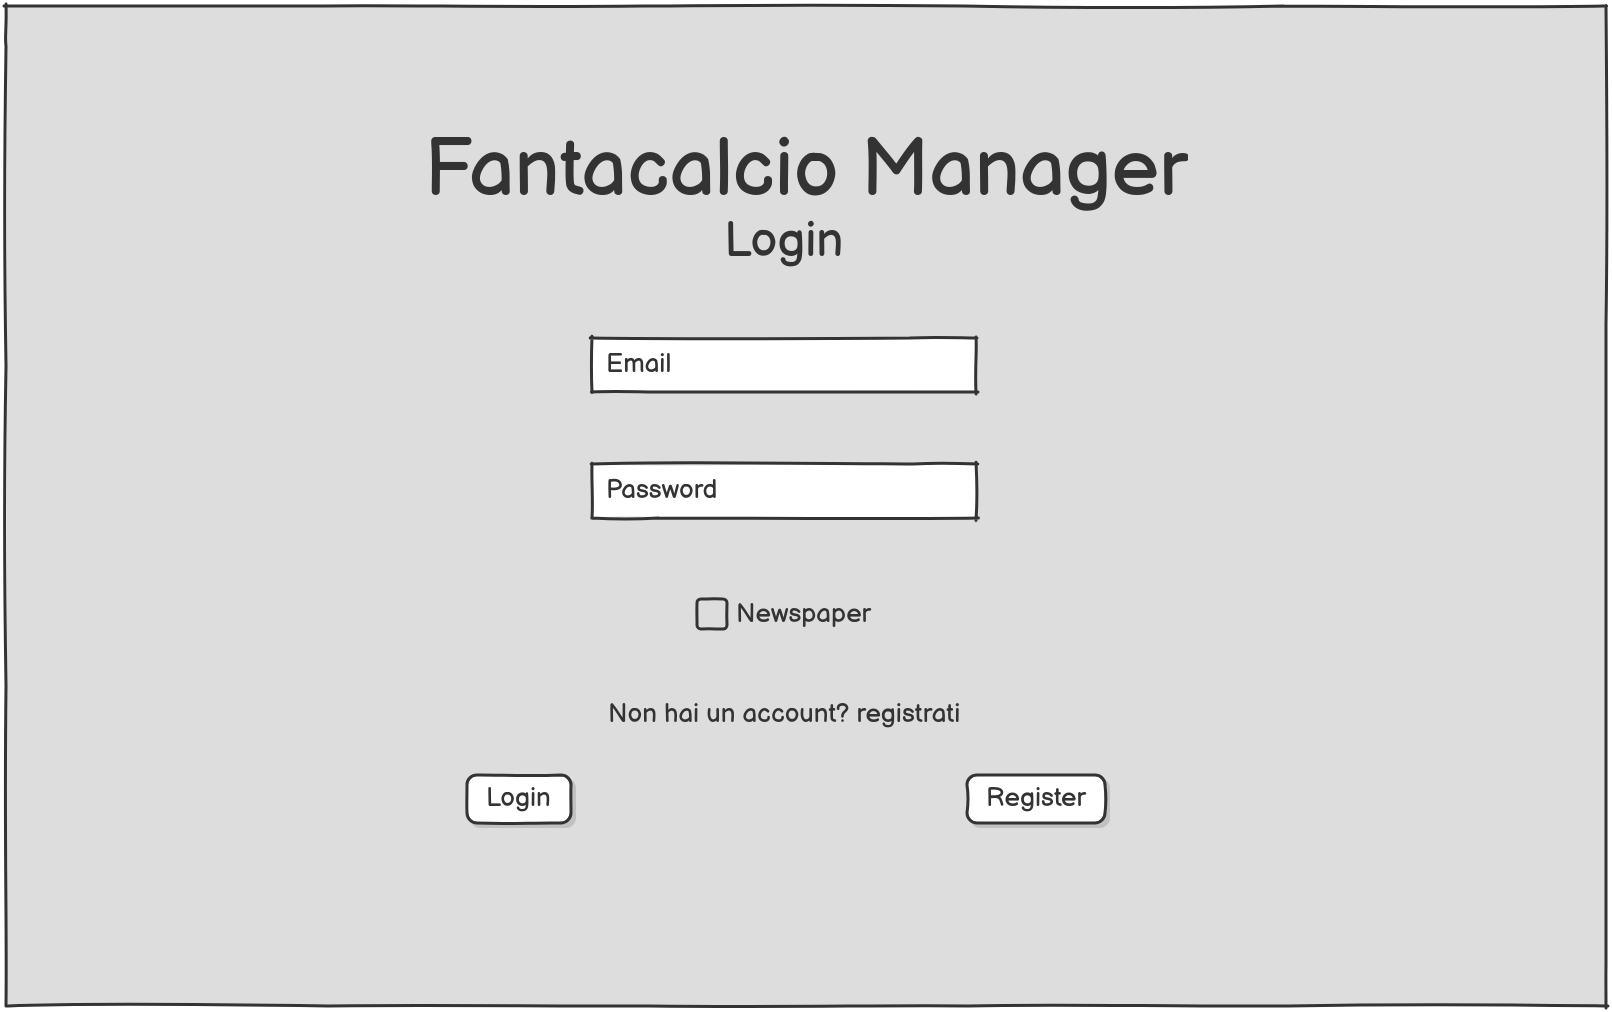
\includegraphics[width=\textwidth]{Resources/Mockups/Login.png}
        \caption{Mockup della pagina di login.}
        \label{fig:pagina_login}
    \end{subfigure}
    \hfill
    \begin{subfigure}[b]{0.49\textwidth}
        \centering
        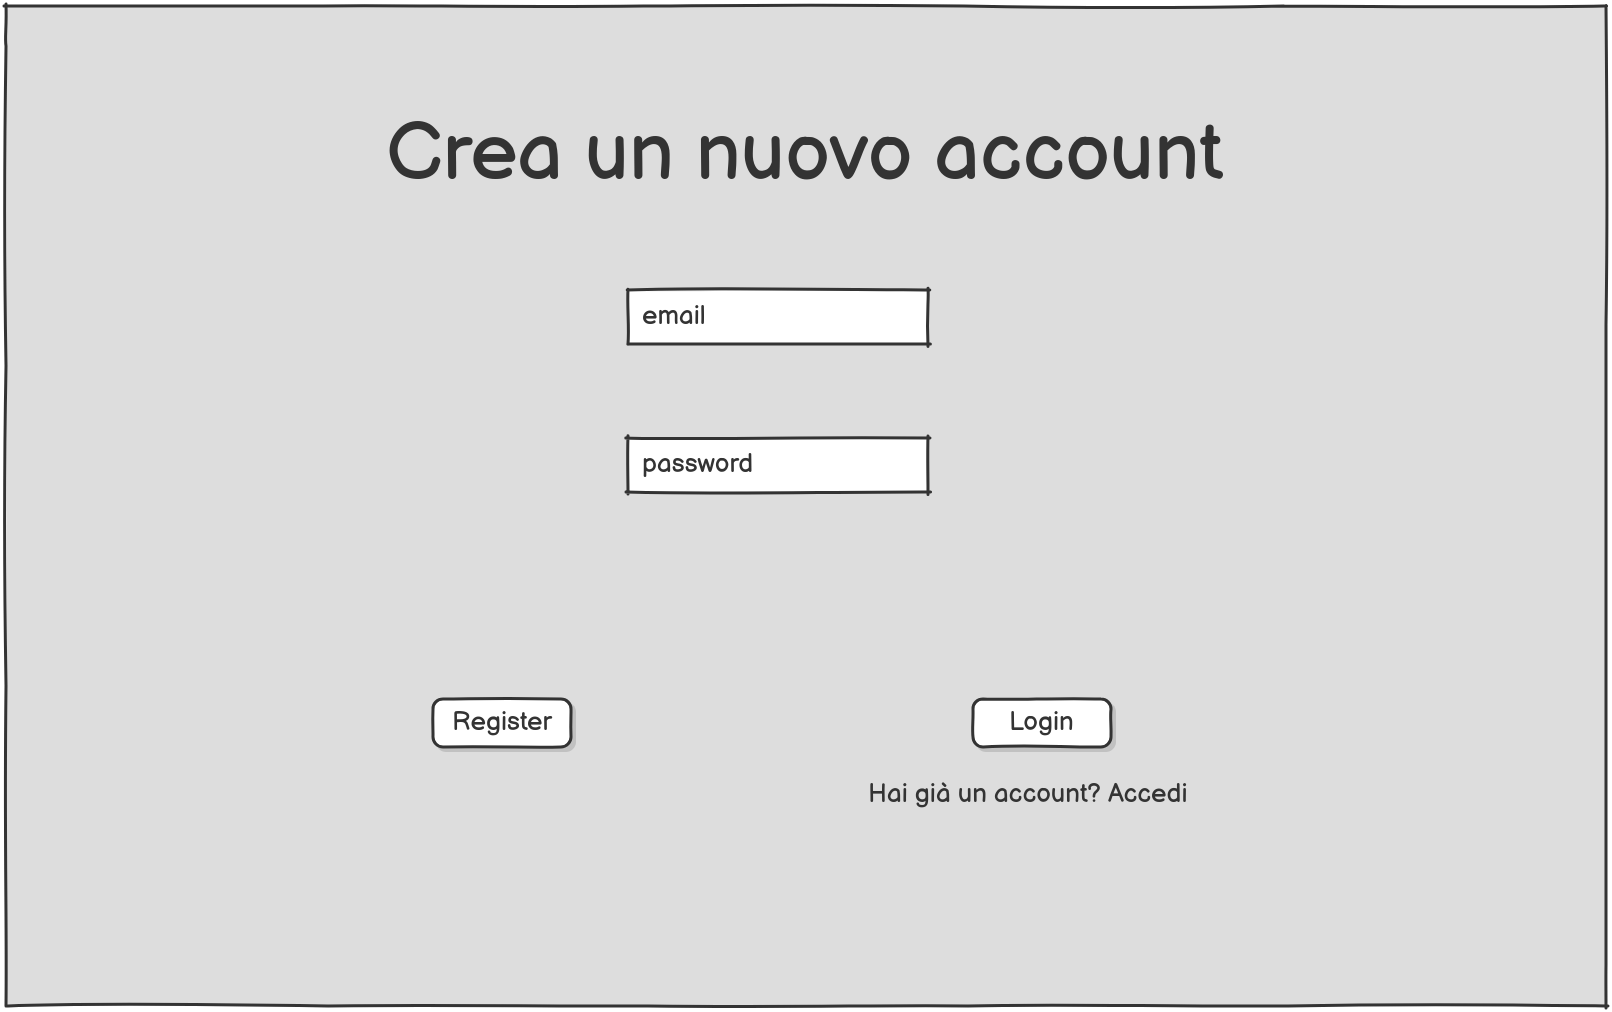
\includegraphics[width=\textwidth]{Resources/Mockups/Registrazione.png}
        \caption{Mockup della pagina di registrazione.}
        \label{fig:pagina_registrazione}
    \end{subfigure}

    % 2ª riga
    \begin{subfigure}[b]{0.49\textwidth}
        \centering
        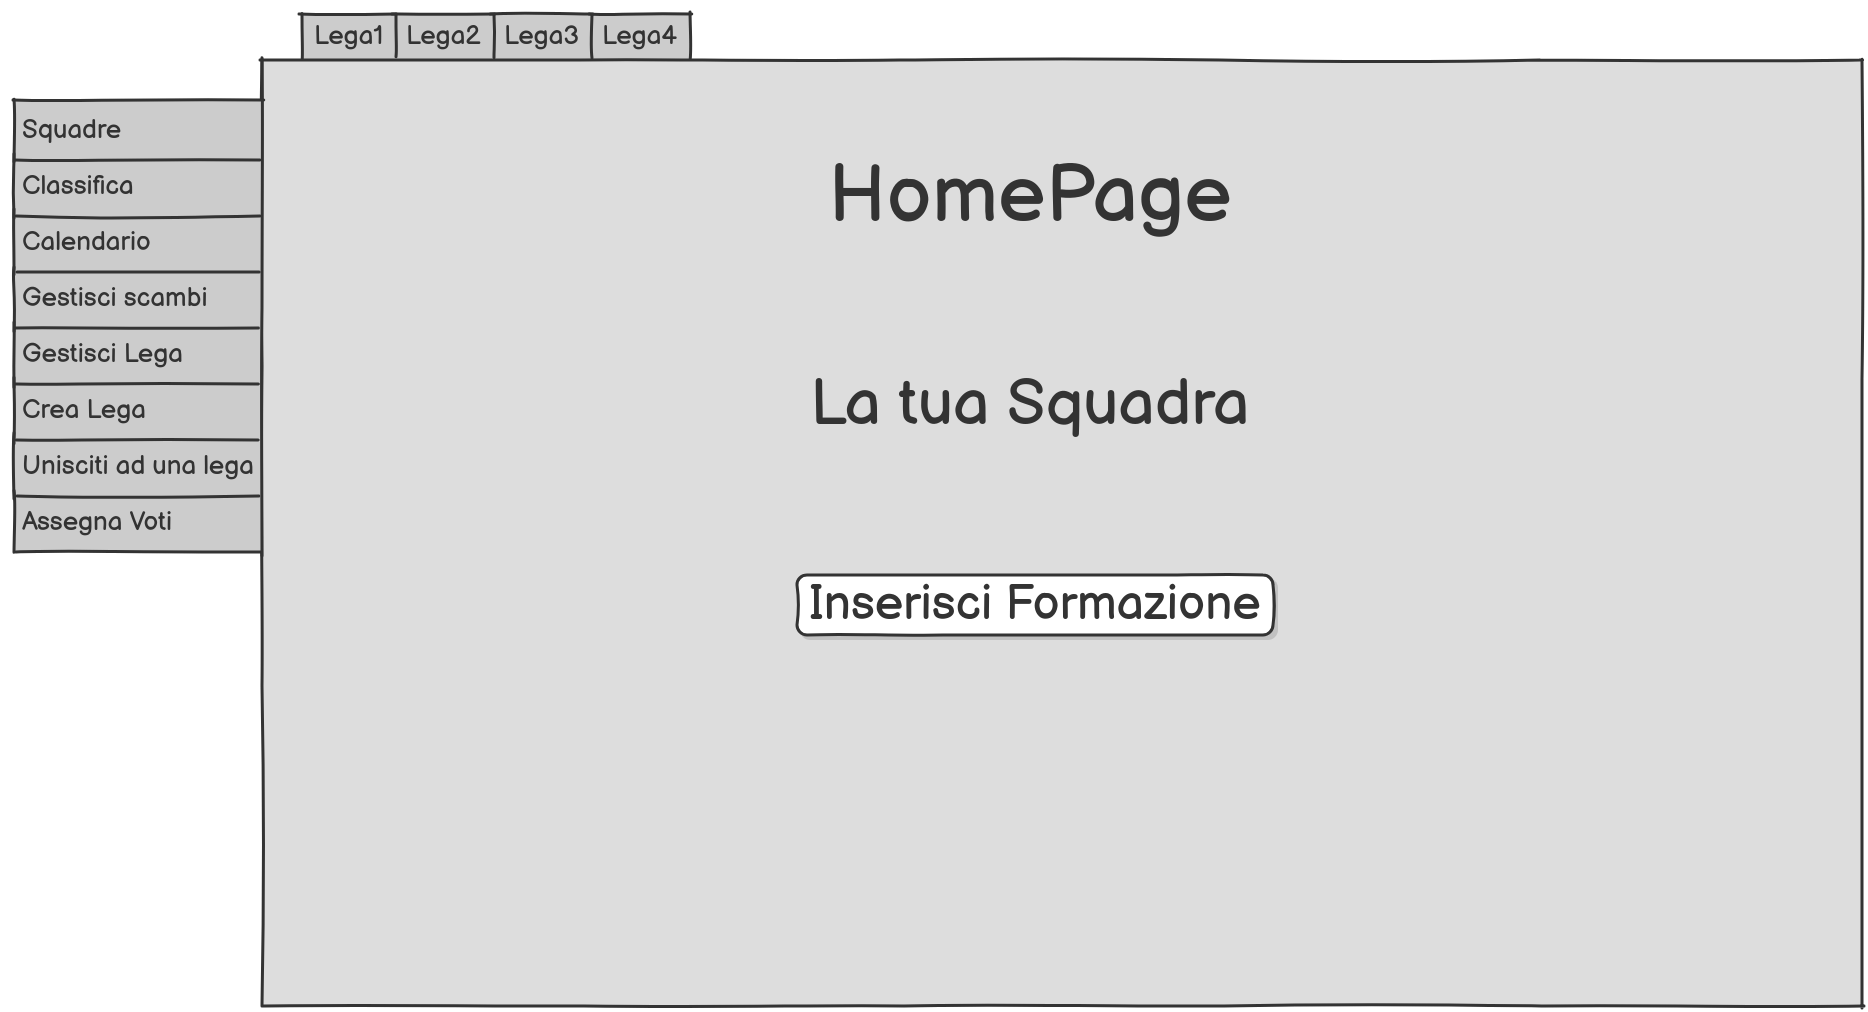
\includegraphics[width=\textwidth]{Resources/Mockups/HomePage.png}
        \caption{Mockup della homepage.}
        \label{fig:pagina_homepage}
    \end{subfigure}
    \hfill
    \begin{subfigure}[b]{0.49\textwidth}
        \centering
        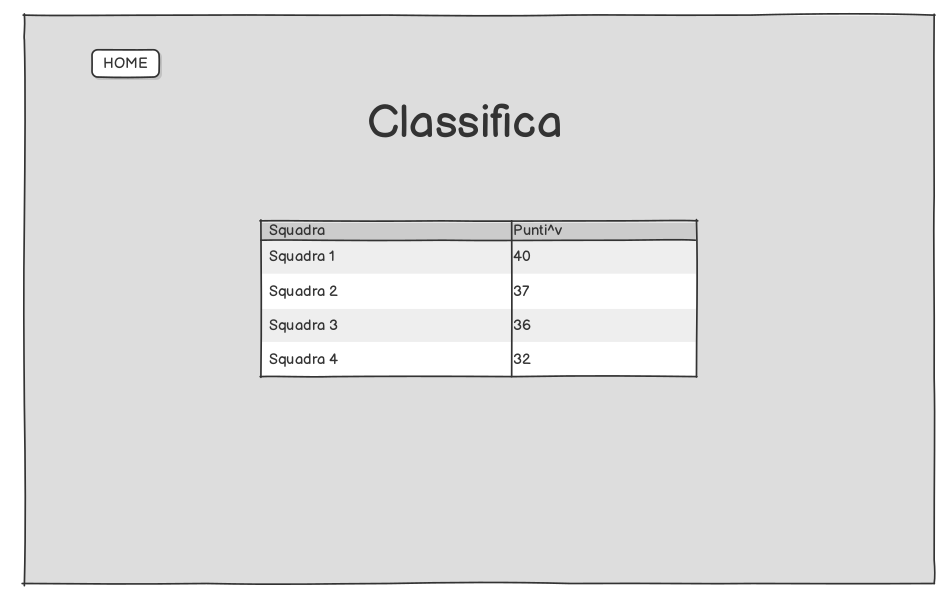
\includegraphics[width=\textwidth]{Resources/Mockups/Classifica.png}
        \caption{Mockup della classifica.}
        \label{fig:pagina_classifica}
    \end{subfigure}

    \caption{Mockup delle pagine di accesso e homepage.}
    \label{fig:mockup_parte1}
\end{figure}
\begin{figure}[H]
    \centering

    % 3ª riga
    \begin{subfigure}[b]{0.49\textwidth}
        \centering
        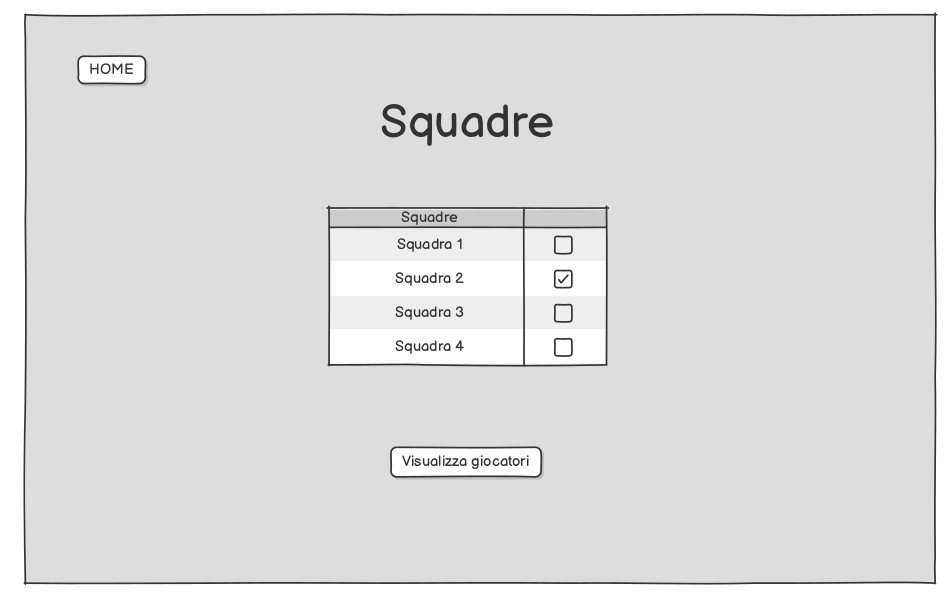
\includegraphics[width=\textwidth]{Resources/Mockups/Squadre.png}
        \caption{Mockup della pagina delle squadre.}
        \label{fig:pagina_squadre}
    \end{subfigure}
    \hfill
    \begin{subfigure}[b]{0.49\textwidth}
        \centering
        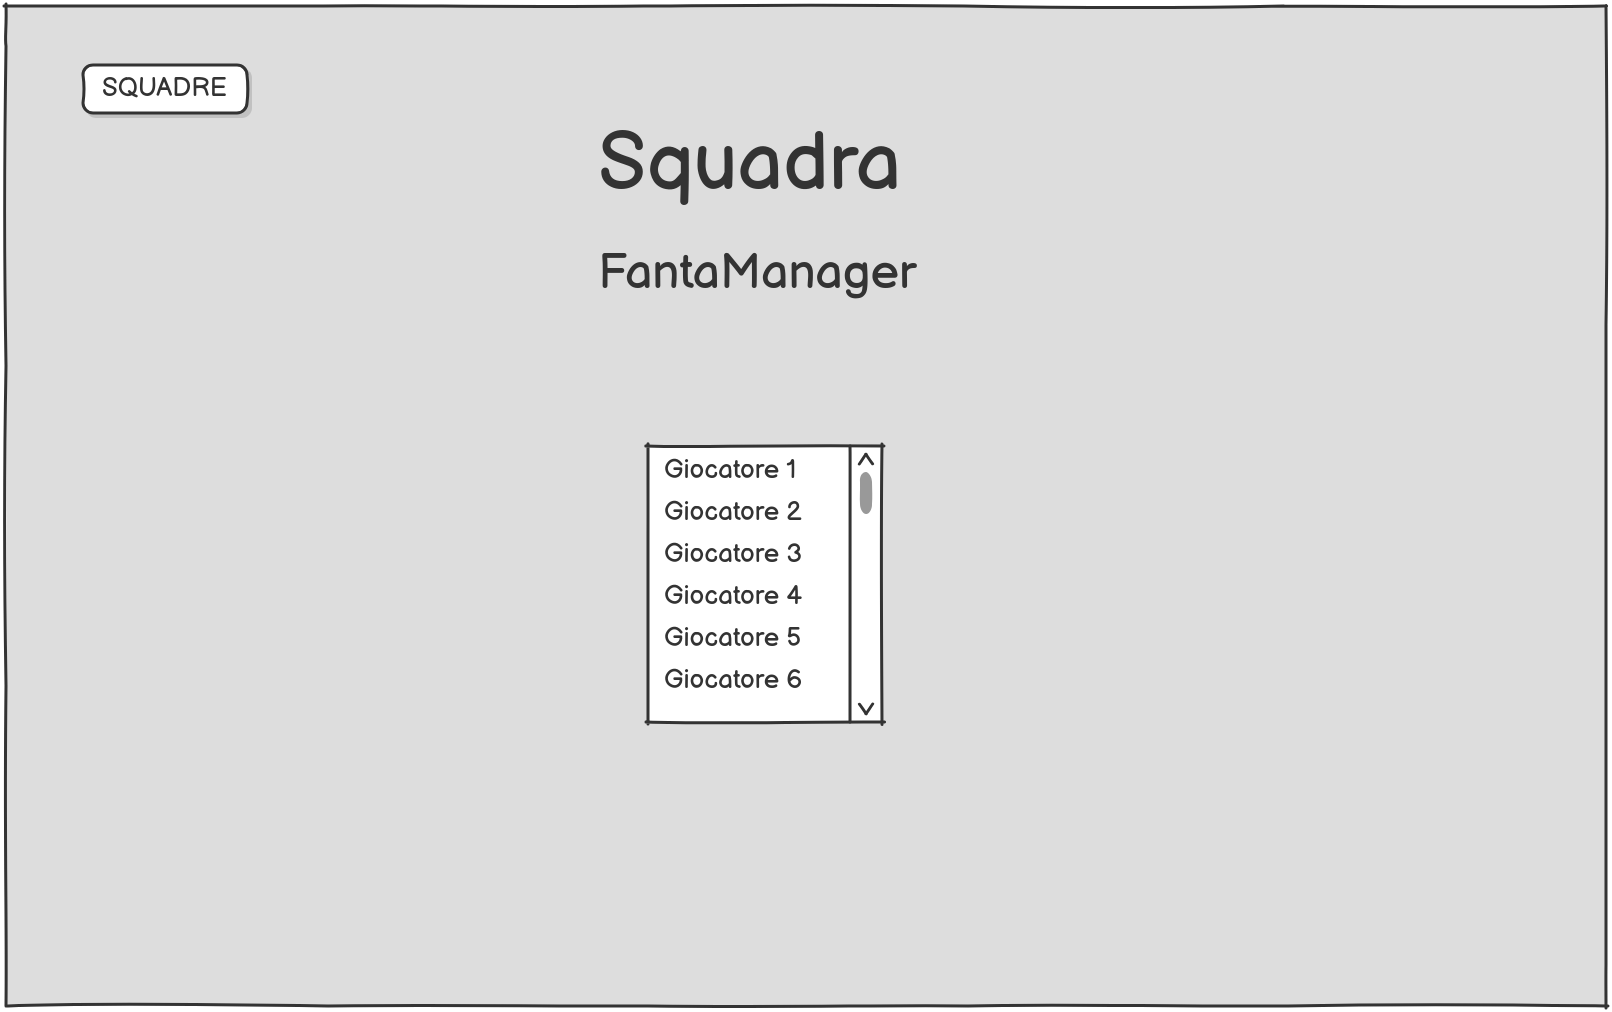
\includegraphics[width=\textwidth]{Resources/Mockups/VisualizzaSquadra.png}
        \caption{Mockup pagina di visualizzazione di un team.}
        \label{fig:pagina_visualizza_squadra}
    \end{subfigure}

    % 4ª riga
    \begin{subfigure}[b]{0.49\textwidth}
        \centering
        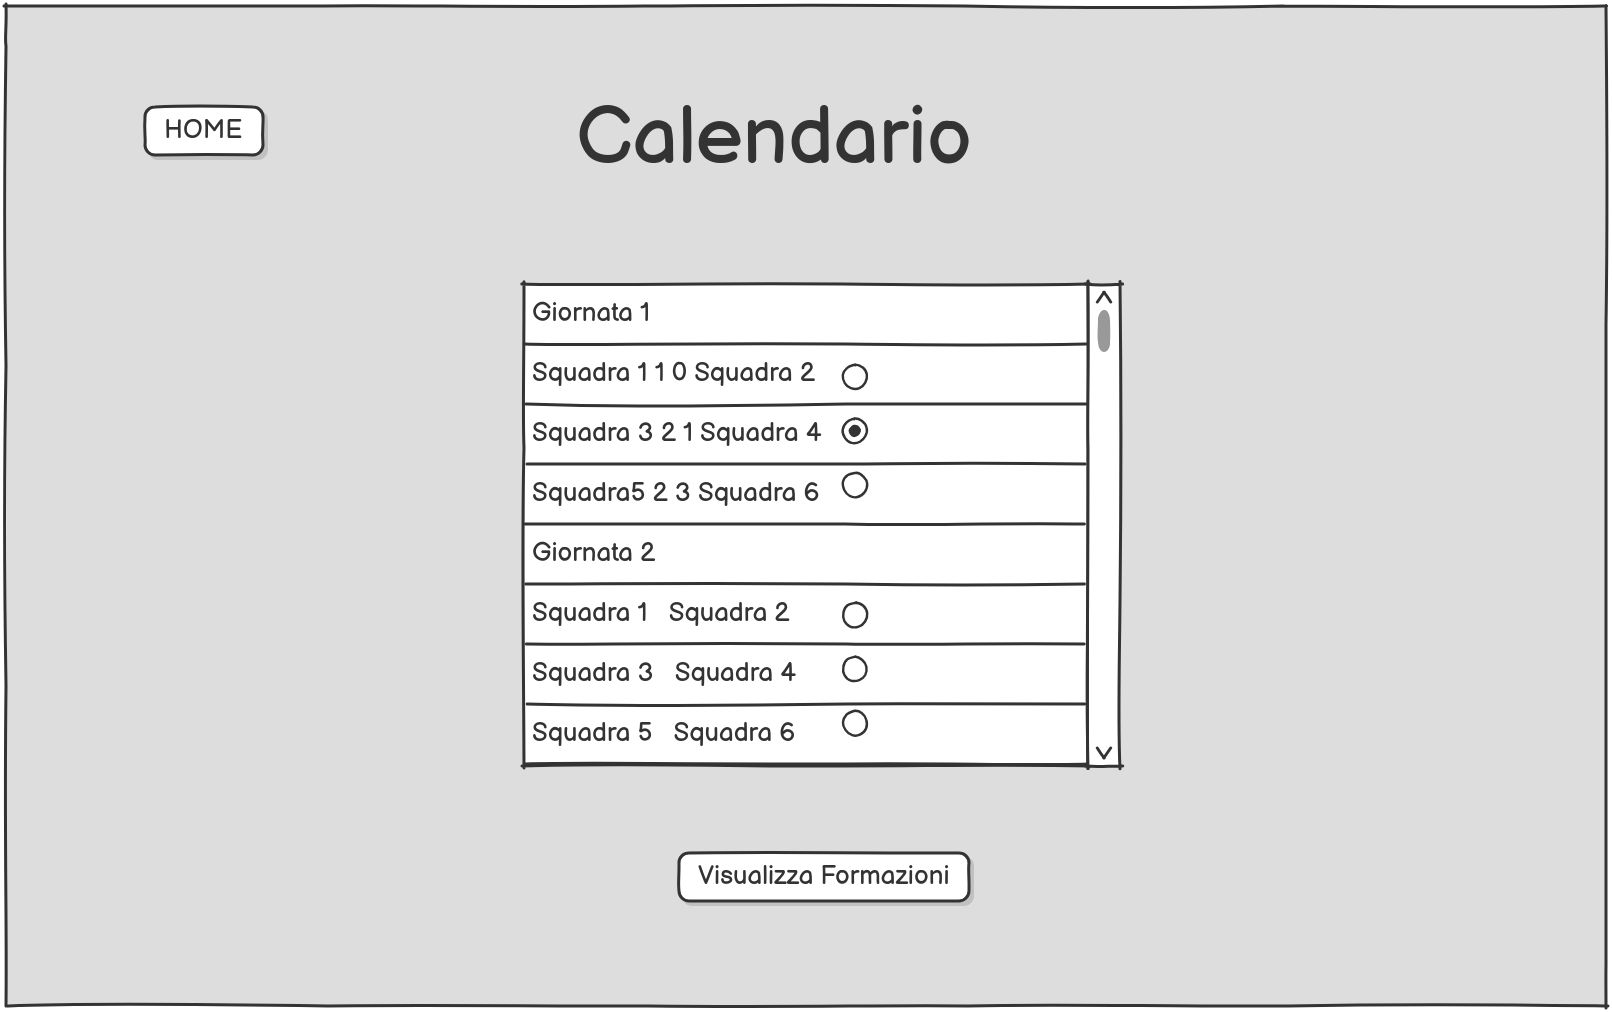
\includegraphics[width=\textwidth]{Resources/Mockups/Calendario.png}
        \caption{Mockup della pagina del calendario.}
        \label{fig:pagina_calendario}
    \end{subfigure}
    \hfill
    \begin{subfigure}[b]{0.49\textwidth}
        \centering
        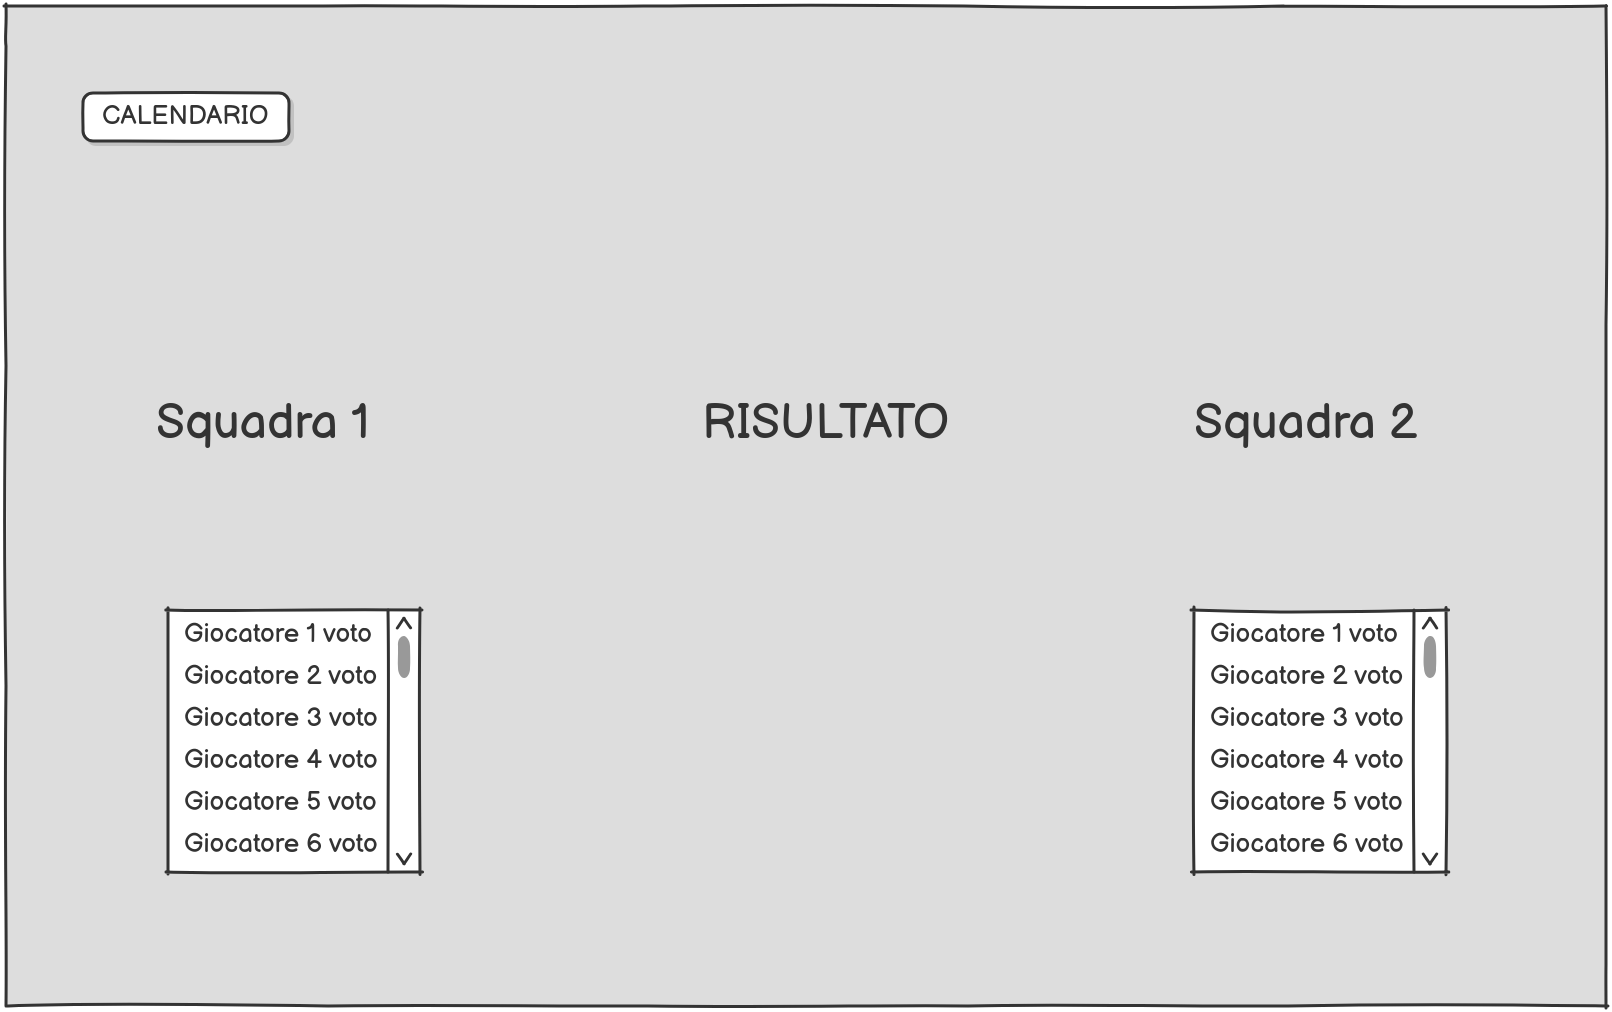
\includegraphics[width=\textwidth]{Resources/Mockups/VisualizzaMatch.png}
        \caption{Mockup pagina di visualizzazione di un match.}
        \label{fig:pagina_visualizza_match}
    \end{subfigure}

    \caption{Mockup delle pagine relative a squadre, calendario e match.}
    \label{fig:mockup_parte2}
\end{figure}
\clearpage
\begin{figure}[H]
    \centering

    % 5ª riga
    \begin{subfigure}[b]{0.49\textwidth}
        \centering
        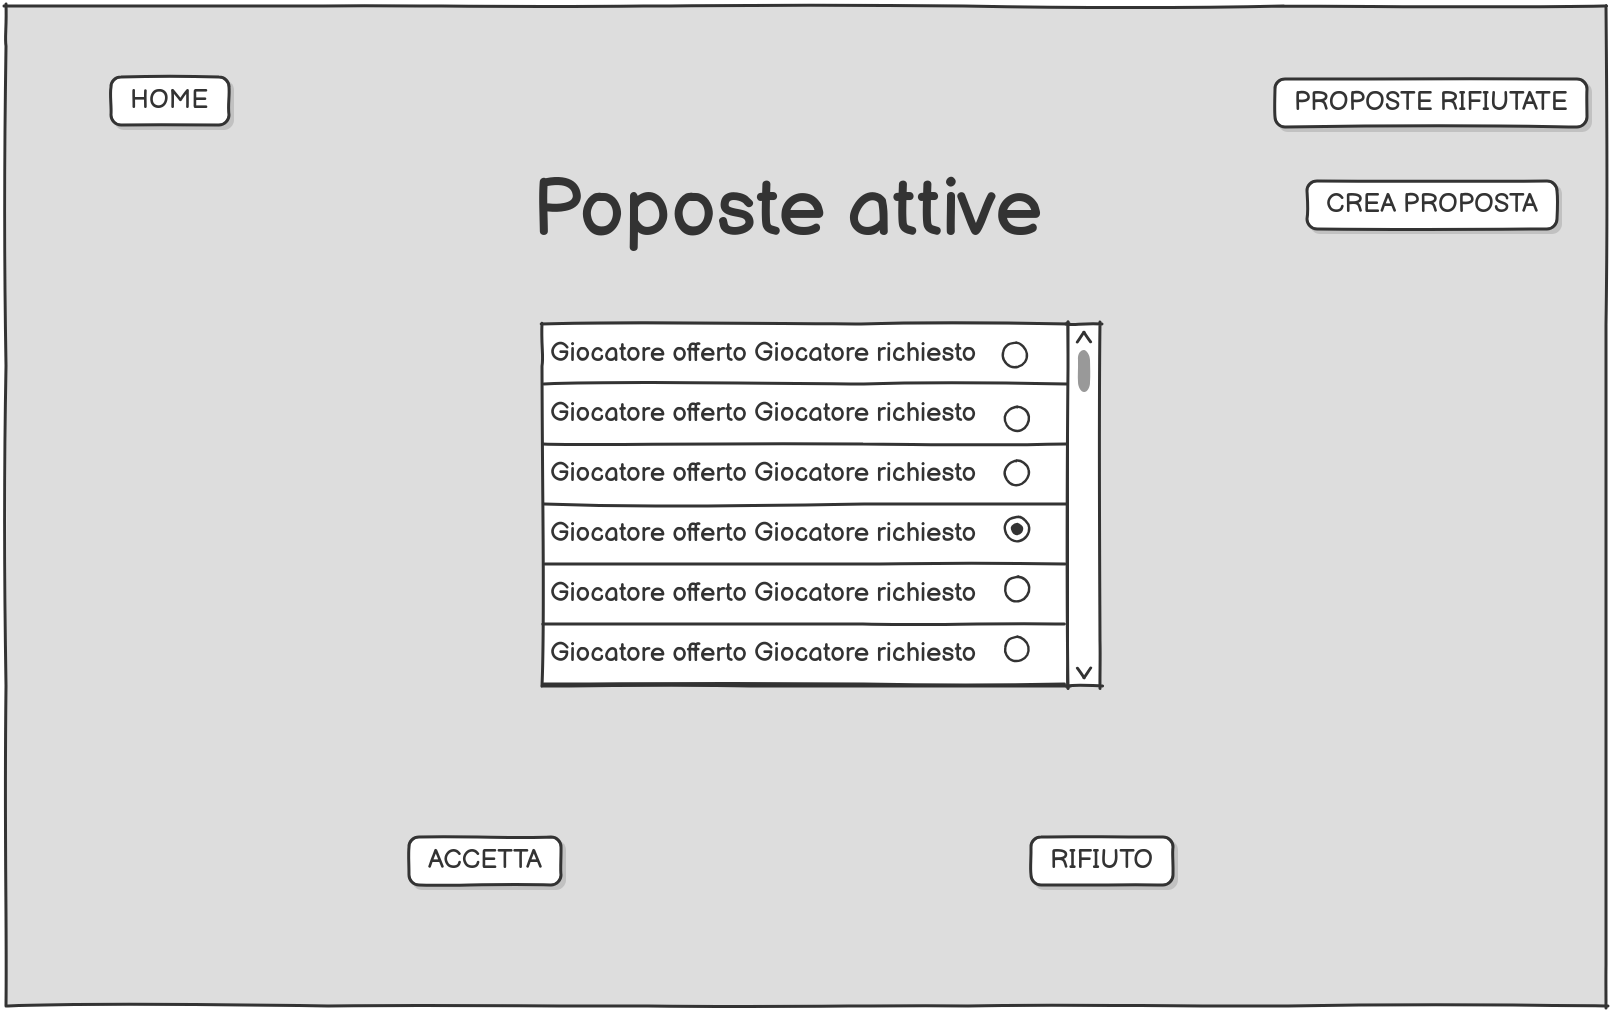
\includegraphics[width=\textwidth]{Resources/Mockups/ProposteAttive.png}
        \caption{Mockup della pagina delle proposte attive.}
        \label{fig:pagina_proposte_attive}
    \end{subfigure}
    \hfill
    \begin{subfigure}[b]{0.49\textwidth}
        \centering
        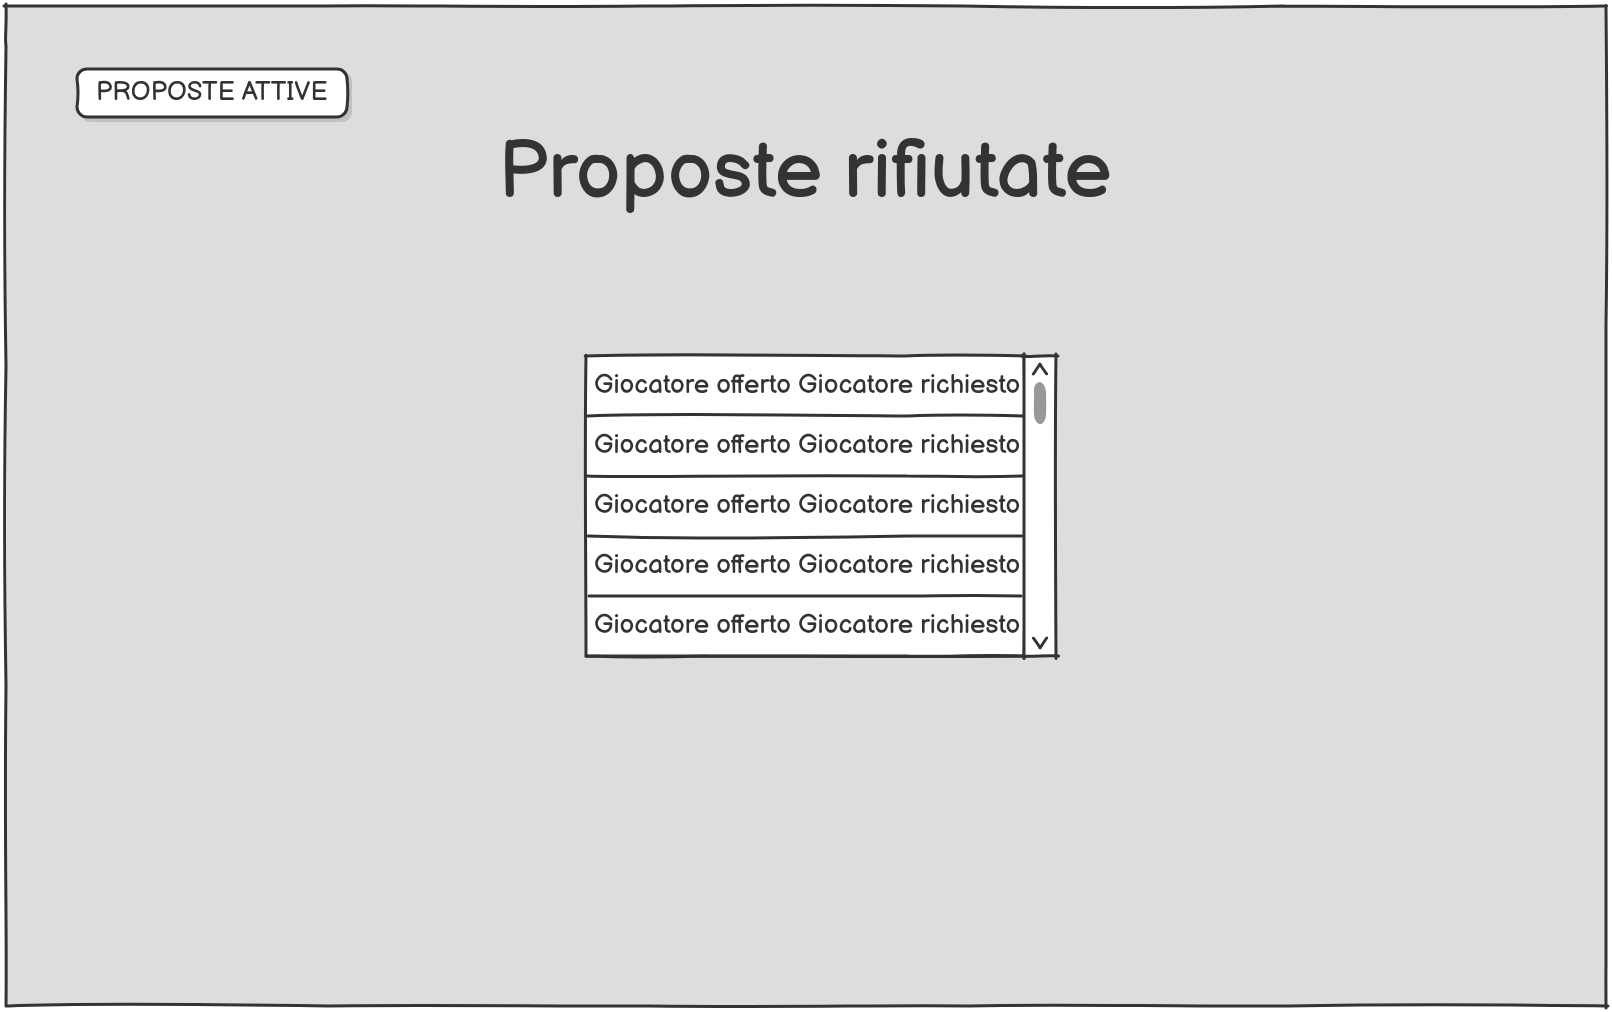
\includegraphics[width=\textwidth]{Resources/Mockups/ProposteRifiutate.png}
        \caption{Mockup della pagina delle proposte rifiutate.}
        \label{fig:pagina_proposte_rifiutate}
    \end{subfigure}

    % 6ª riga
    \begin{subfigure}[b]{0.49\textwidth}
        \centering
        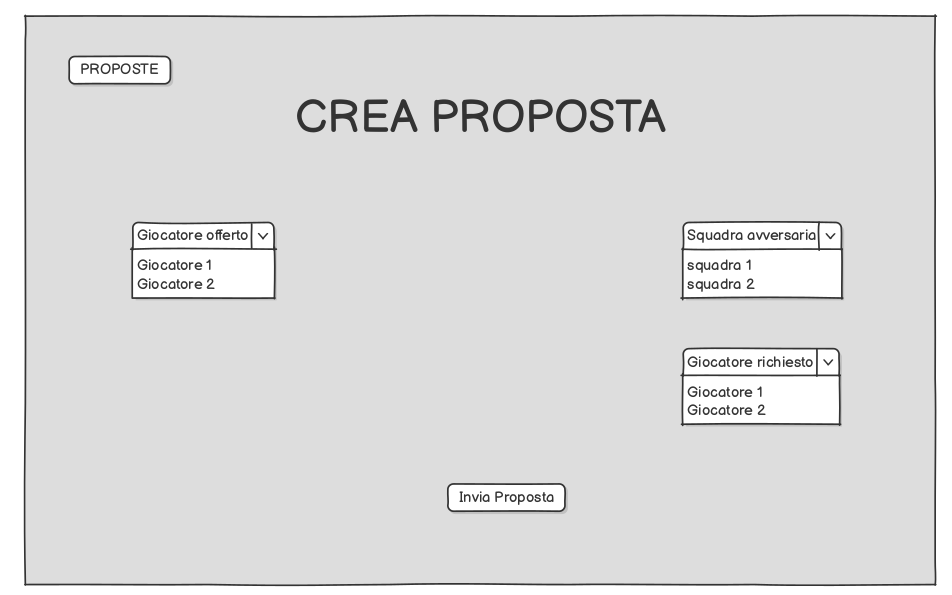
\includegraphics[width=\textwidth]{Resources/Mockups/CreaProposta.png}
        \caption{Mockup pagina per la creazione delle proposte.}
        \label{fig:pagina_crea_proposta}
    \end{subfigure}
    \hfill
    \begin{subfigure}[b]{0.49\textwidth}
        \centering
        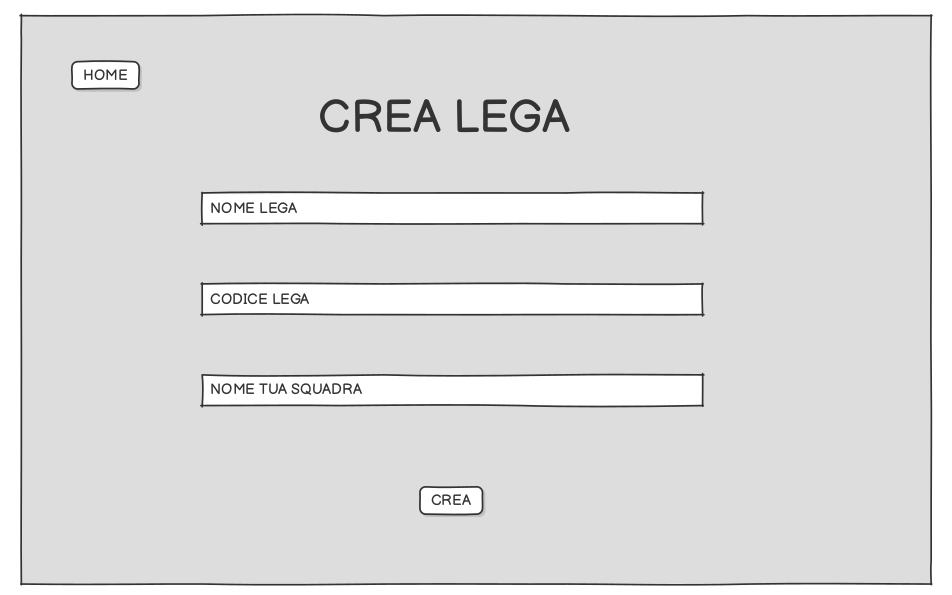
\includegraphics[width=\textwidth]{Resources/Mockups/CreaLega.png}
        \caption{Mockup della pagina di creazione di una lega.}
        \label{fig:pagina_crea_lega}
    \end{subfigure}

    \caption{Mockup delle pagine relative a proposte e creazione di leghe.}
    \label{fig:mockup_parte3}
\end{figure}
\begin{figure}[H]
    \centering

    % 7ª riga
    \begin{subfigure}[b]{0.49\textwidth}
        \centering
        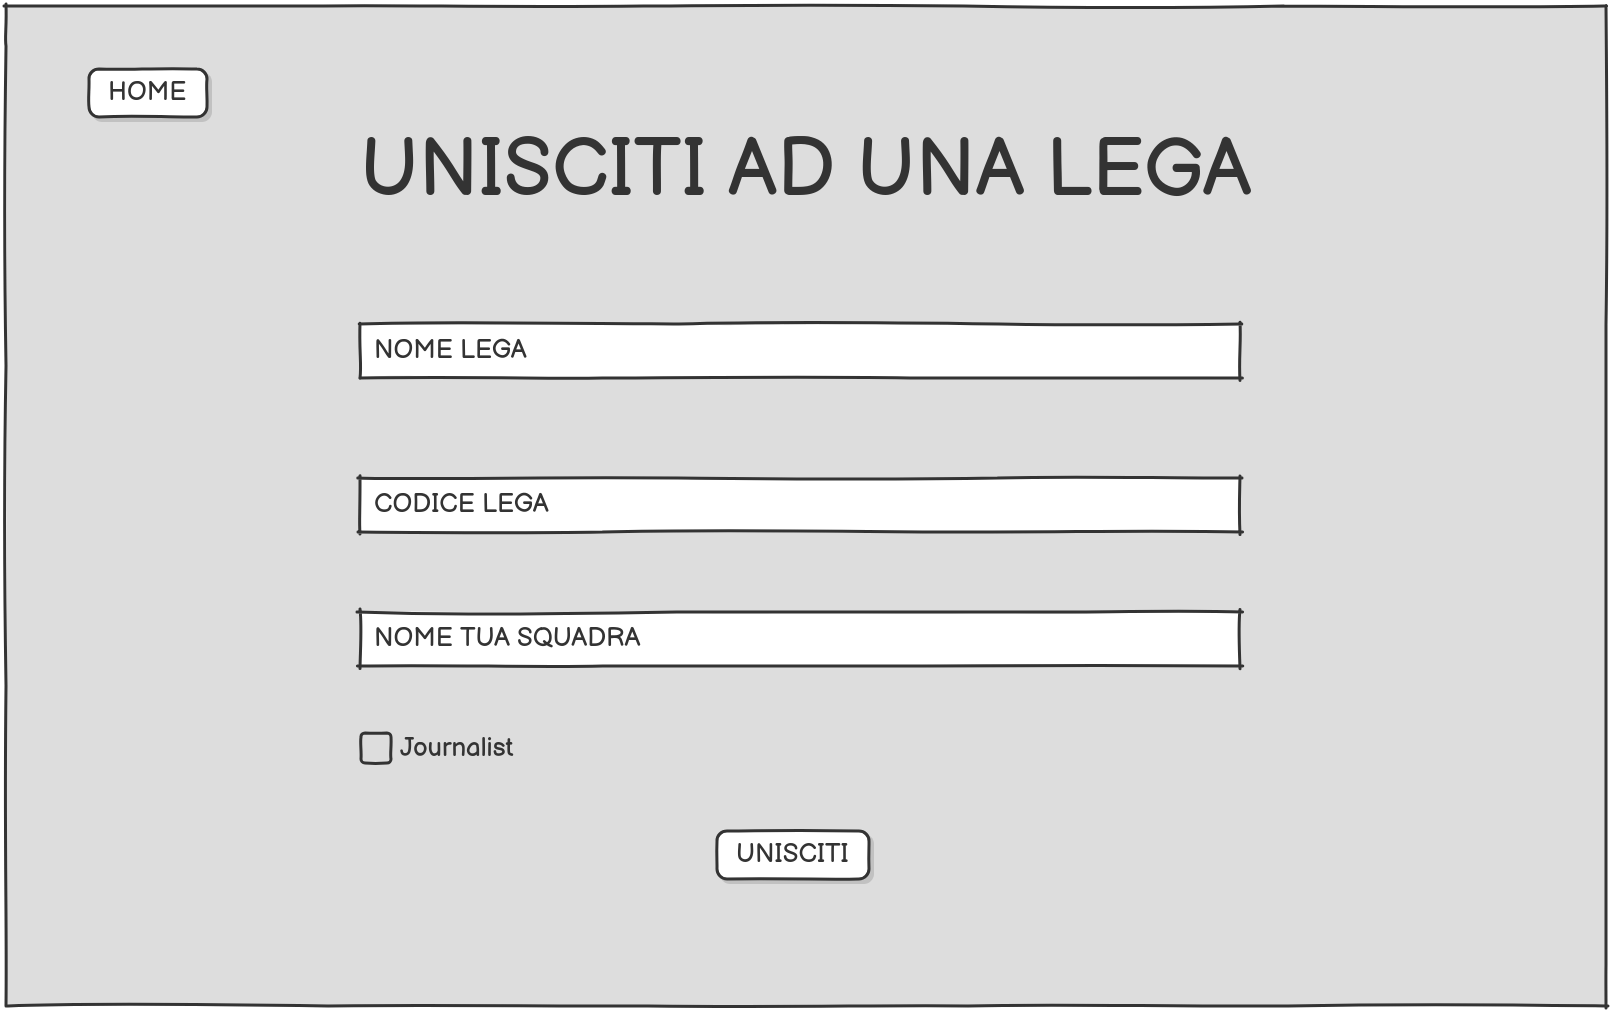
\includegraphics[width=\textwidth]{Resources/Mockups/UniscitiAdUnaLega.png}
        \caption{Mockup della pagina per l'adesione a una lega.}
        \label{fig:pagina_unisciti_lega}
    \end{subfigure}
    \hfill
    \begin{subfigure}[b]{0.49\textwidth}
        \centering
        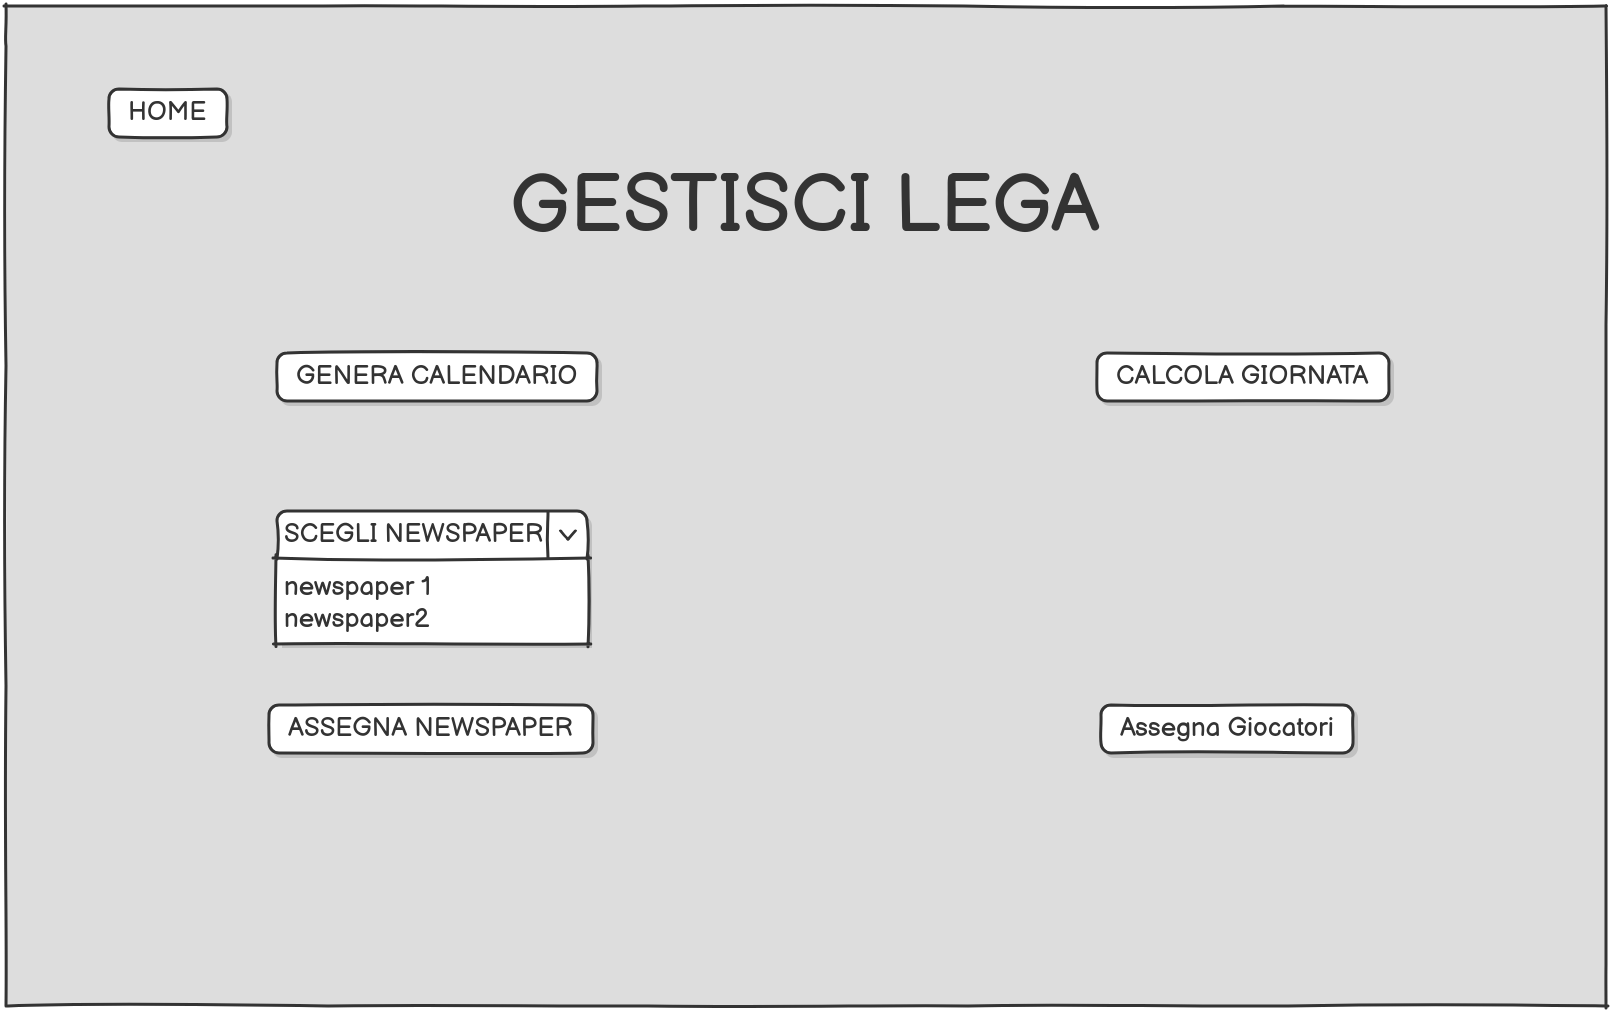
\includegraphics[width=\textwidth]{Resources/Mockups/GestisciLega.png}
        \caption{Mockup della pagina per la gestione della lega.}
        \label{fig:pagina_gestisci_lega}
    \end{subfigure}

    % 8ª riga
    \begin{subfigure}[b]{0.49\textwidth}
        \centering
        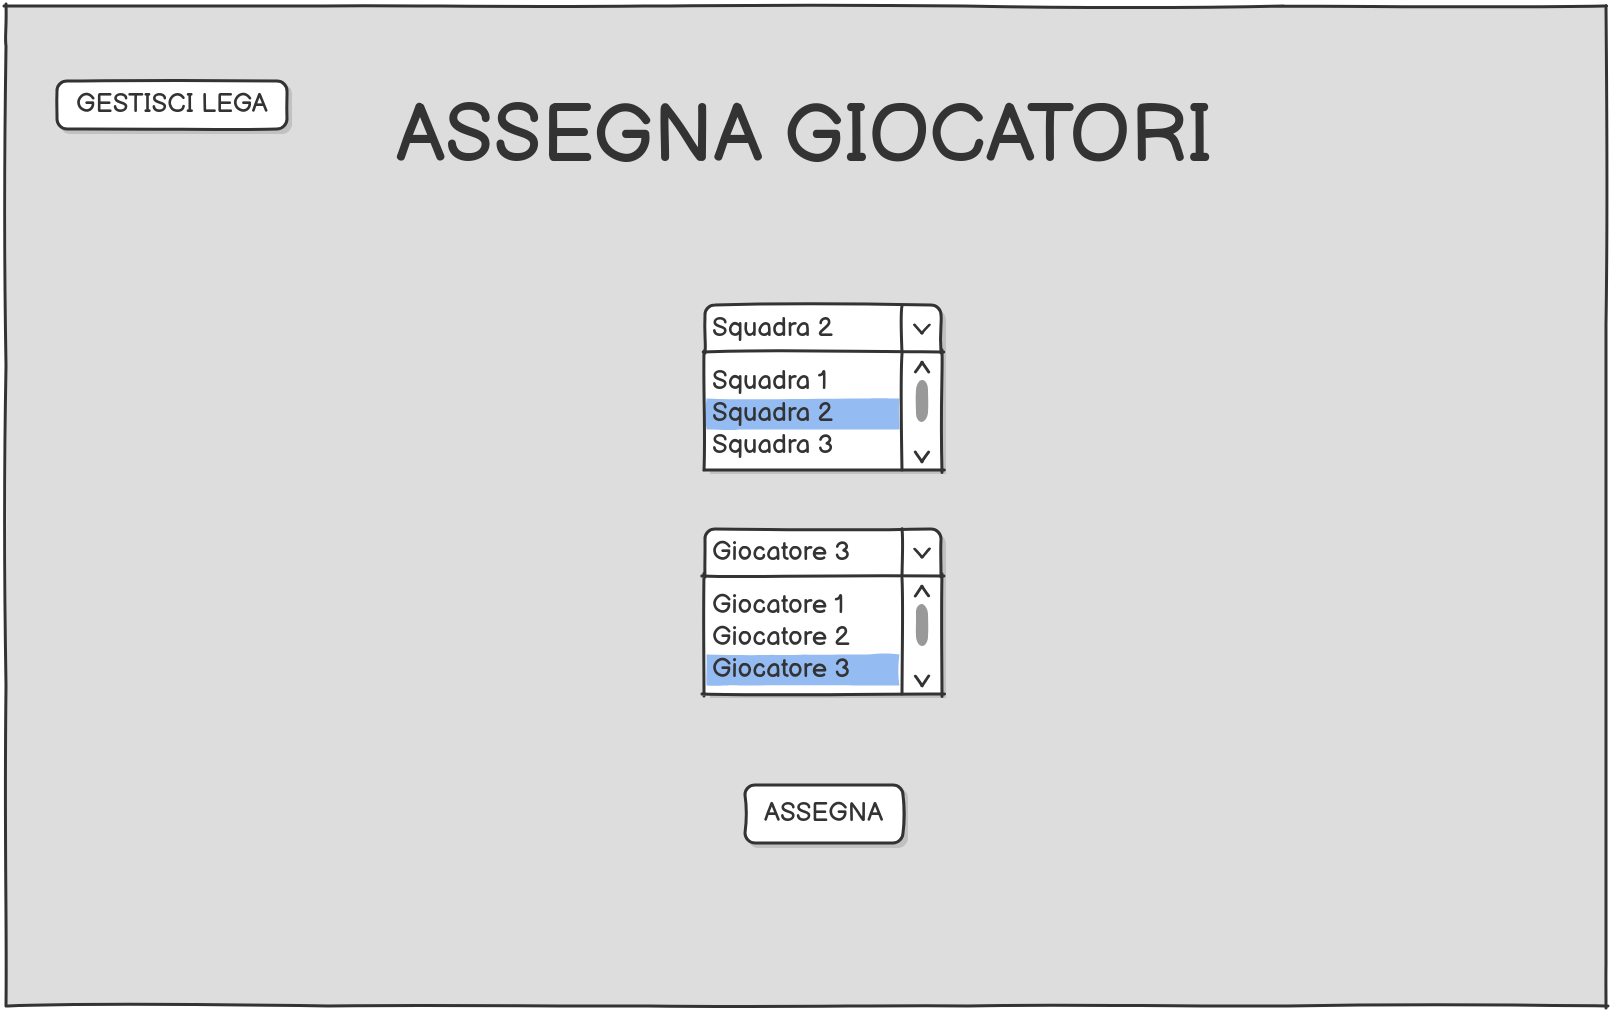
\includegraphics[width=\textwidth]{Resources/Mockups/AssegnaGiocatori.png}
        \caption{Mockup pagina assegnazione dei giocatori ai team.}
        \label{fig:pagina_assegna_giocatori}
    \end{subfigure}
    \hfill
    \begin{subfigure}[b]{0.49\textwidth}
        \centering
        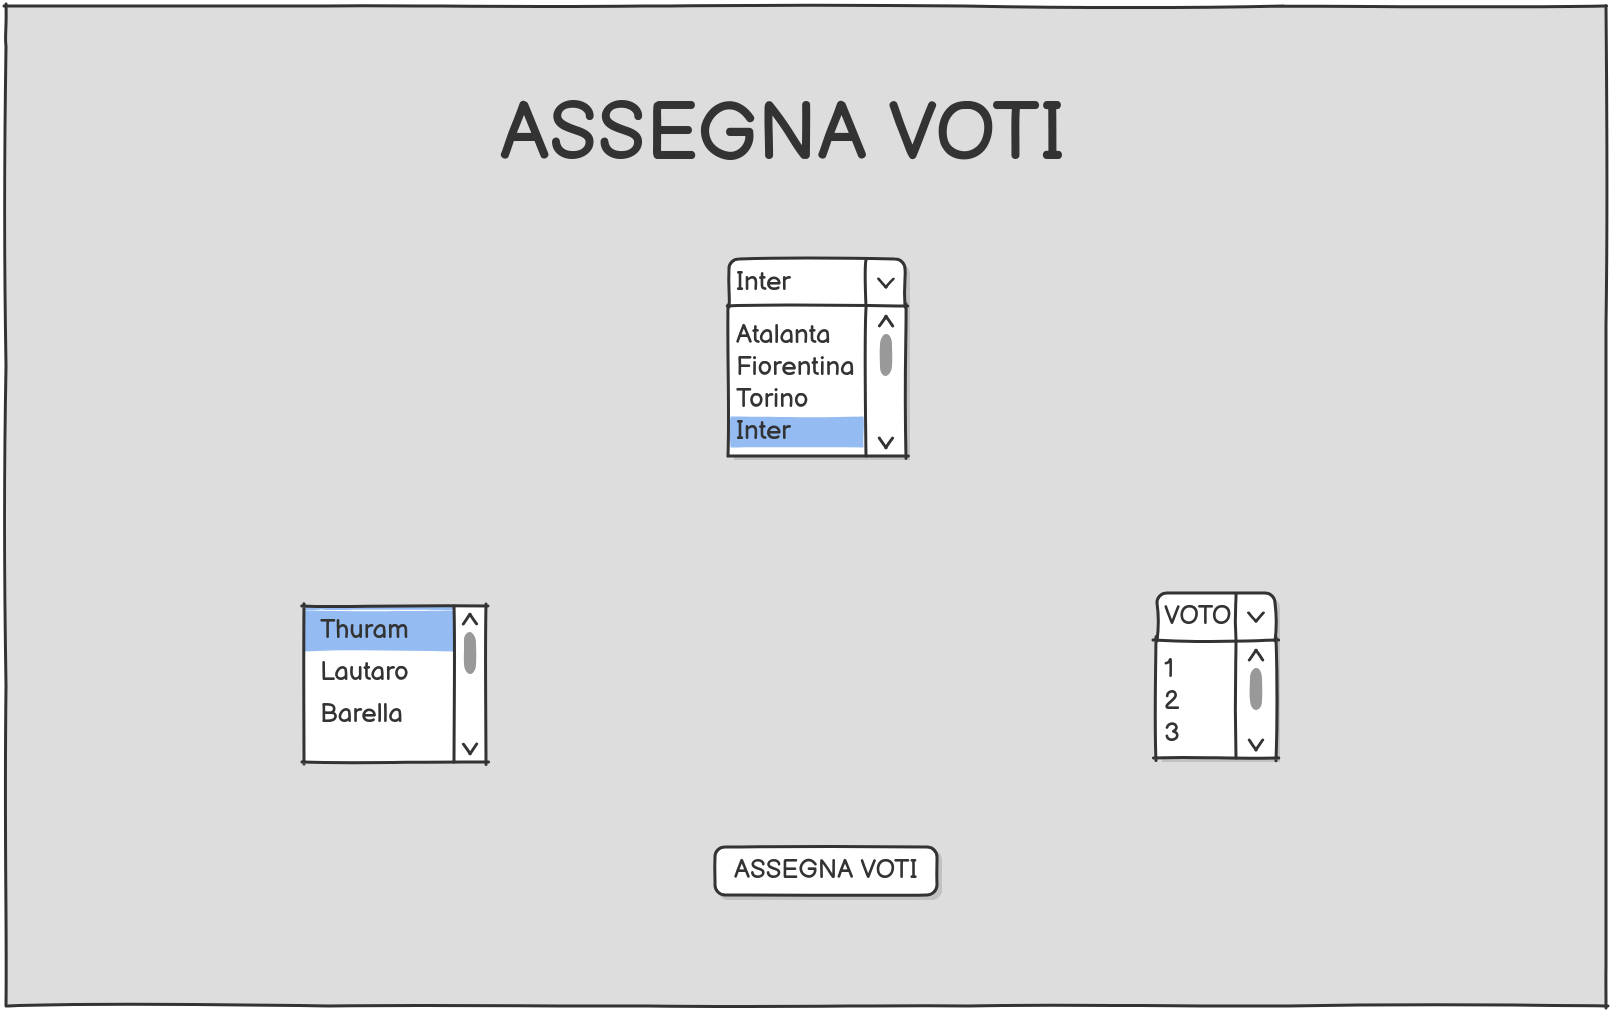
\includegraphics[width=\textwidth]{Resources/Mockups/AssegnaVoti.png}
        \caption{Mockup della pagina per l'assegnazione dei voti.}
        \label{fig:pagina_assegna_voti}
    \end{subfigure}

    \caption{Mockup delle pagine di gestione delle leghe e assegnazioni.}
    \label{fig:mockup_parte4}
\end{figure}
